\documentclass{article}
\usepackage[gobble=auto]{pythontex}
\usepackage{amsmath}
\usepackage{amssymb}
\usepackage{bm}
\usepackage{bbm}
\usepackage{graphicx}

\fvset{breaklines}
\renewcommand\thesubsection{\alph{subsection}}

\title{CSC311 - Final Assignment}
\author{Zelong Liu, Fizzah Mansoor, Harrison Deng}



\pylabc[KNN]{pytex.add_dependencies("./knn.py")}
\pylabc[IRT]{pytex.add_dependencies("./item_response.py")}
\pylabc[NN]{pytex.add_dependencies("./neural_network.py")}
\pylabc[ENSEMBLE]{pytex.add_dependencies("./ensemble.py")}

\begin{document}

    \maketitle

    \pagebreak

    \tableofcontents

    \pagebreak
    
    \part{Predicting Student Correctness}
    
    \section{K-Nearest Neighbor}

    Following parts will refer to the following information:

    \begin{pylabblock}[KNN]
        import knn as knn
        k_vals, val_user_acc, val_item_acc = knn.main(data_path="./data")
    \end{pylabblock}

    Output:
    
    \printpythontex[verb]

    \subsection{Complete Main kNN, Plot and Report Accuracy}
    The implementation of all code is in the \verb|part_a/knn.py| file. Following are plots of accuracy on validation data as a function of $k \in \{1,6,11,16,21,26\}$:

    \begin{pylabblock}[KNN]
        knn.accuracy_plot(k_vals, val_user_acc, "User-Based Collaborative Filtering")
    \end{pylabblock}

    \includegraphics[scale=0.7]{figures/generated/knn_User-Based_Collaborative_Filtering.pdf}

    See accuracies in the data output near the beginning of the question.


    \subsection{Selecting k*}
    We selected $k=11$ for user-based collaborative filtering as this resulted in the highest validation accuracy (refer to data output of \verb|main| function near beginning of question for report on final test accuracy).
    
    \subsection{Implementing Impute by Item}
    The implementation is in the same file as the user-based version.

    Underlying assumption: if answers by certain users to Question A match those of Question B, then A’s answer correctness corresponding to a specific user matches that of question Y. 

    Repetition of a) and b) where the data is in the same output box as for user-based collaborative filtering and plot as follows:

    \begin{pylabblock}[KNN]
        knn.accuracy_plot(k_vals, val_item_acc, "Item-Based Collaborative Filtering")
    \end{pylabblock}

    \includegraphics[scale=0.70]{figures/generated/knn_Item-Based_Collaborative_Filtering.pdf}    

    \subsection{Comparing user and item based Collaborative Filtering}
    User-Based collaborative filtering performs better on test data. $68.416\%$ accuracy on user-based filtering and $68.162\%$ accuracy on item-based filtering.

    \subsection{Potential Limitations of kNN in this Context}
    We can safely assume that there is a high correlation between both question difficulty and student ability on whether or not the question was answered correctly. But, feature importance is not possible for the KNN algorithm (there is no way to define the features which are responsible for the classification), so it will not be able to make accurate inferences based on these two parameters. In the algorithm used in this question, either one of the two parameters (user ability or question difficulty) is focused on, so it has lower validation and test accuracy scores than other algorithms in Part A of this project. 

    KNN runs slowly. Finding the optimal k-value from the given list of possible k values ({1, 6, 11, 21, 26}) takes several minutes for each function.

    
    \pagebreak

    \section{Item Response Theory}
    \subsection{Mathematical Derivations for IRT}
    We are given that $p(c_{ij} = 1 \vert \bm{\theta}, \bm{\beta})$. We will assume $c_{ij}$ is a value in $\bm{C}$ where $i$ and $j$ as coordinates are in set $O$ as defined:
    \[ O = \{(i,j): \text{Entry $(i,j)$ of matrix $\bm{C}$ and is observed}\} \].

    Since this $c_{ij}$ is a binary value, we can describe $P(\bm{C} \vert \bm{\theta}, \bm{\beta})$ with a bernoulli distribution:
    \[p(C \vert \bm{\theta}, \bm{\beta}) = \prod_{ij}[\frac{exp(\theta_{i} - \beta_{j})}{1+exp(\theta_{i} - \beta_{j})}]^{c_{ij}}[\frac{1}{1 + exp(\theta_{i} - \beta_{j})}]^{(1-c_{ij})}\]

    Therefore, our Likelihood function is:
    \[L(\bm{\theta}, \bm{\beta}) =\prod_{ij}[\frac{exp(\theta_{i} - \beta_{j})}{1+exp(\theta_{i} - \beta_{j})}]^{c_{ij}}[\frac{1}{1 + exp(\theta_{i} - \beta_{j})}]^{(1-c_{ij})}\]

    Then, apply log to obtain the log-likelihood where $N$ and $M$ are the number of users and questions respectively:
    \begin{align*}
        L(\bm{\theta}, \bm{\beta}) &=\prod_{ij}[\frac{exp(\theta_{i} - \beta_{j})}{1+exp(\theta_{i} - \beta_{j})}]^{c_{ij}}[\frac{1}{1 + exp(\theta_{i} - \beta_{j})}]^{(1-c_{ij})} \\
        log(L(\bm{\theta}, \bm{\beta})) &= \log(\prod_{ij}[\frac{exp(\theta_{i} - \beta_{j})}{1+exp(\theta_{i} - \beta_{j})}^{c_{ij}}][\frac{1}{1 + exp(\theta_{i} - \beta_{j})}^{1-c_{ij}}] \\
        &=\sum_{i=1}^{N} \sum_{j=1}^{M} \log([\frac{exp(\theta_{i} - \beta_{j})}{1+exp(\theta_{i} - \beta_{j})}^{c_{ij}}][\frac{1}{1 + exp(\theta_{i} - \beta_{j})}^{1-c_{ij}}]) \\
        &=\sum_{i=1}^{N} \sum_{j=1}^{M} c_{ij}((log(exp(\theta_{i} - \beta_{j})) - log(1 + exp(\theta_{i} - \beta_{j}))) \\
        &+ (1 - c_{ij})(\log(1) - \log(1 + exp(\theta_{i} - \beta_{j}))) \\
        &=\sum_{i=1}^{N} \sum_{j=1}^{M} [c_{ij}(\theta_{i} - \beta_{j}) - \log(\frac{exp(\theta_{i} - \beta_{j})}{1+exp(\theta_{i} - \beta_{j})})] \\
    \end{align*}

    Then, we solve for the partial derivative with respect to $\theta_i$ and $\beta_j$ respectively:
    \begin{align*}
        \frac{\delta}{\delta\theta_{i}} &=  \sum_{j=1}^{M}{[c_{ij} - \frac{exp(\theta_{i} - \beta_{j})}{1+exp(\theta_{i} - \beta_{j})}]} \\
        \frac{\delta}{\delta\beta_{j}} &= \sum_{i=1}^{N}{[-c_{ij} + \frac{exp(\theta_{i} - \beta_{j})}{1+exp(\theta_{i} - \beta_{j})}]}
    \end{align*}
    
    \subsection{Implementation of IRT}
    The implementation of IRT is in \verb|part_a/item_response.py|. We chose the hyperparameters $\alpha$ and iterations number by performing multiple combinations of them and seeing which one had the highest validation score (automated, see mentioned code file for this automation). We then manually adjusted the set of tested values and repeated. Doing this a few times resulted in:

    \begin{pylabblock}[IRT]
        import item_response as irt
        print()
        irt_results = irt.main("./data")
    \end{pylabblock}
    \printpythontex[verb]

    Which is the best result out of the combinations we tried.

    The following is the training curve showing training and validation negative log likelihoods as a function of number of iterations:

    \includegraphics[scale=0.7]{figures/generated/irt_Neg_Log_Likelihood_for_Train_and_Validation_Data.pdf}

    \medskip

    \subsection{Reporting Validation and Test Accuracies}

    Validation and test accuracies have been calculated in the previous call to the main function. Implementation is in \verb|part_a/item_response.py|.

    \medskip

    \noindent
    Our validation accuracy:
    \begin{pylabblock}[IRT]
        print(irt_results["val_acc"])
    \end{pylabblock}
    \printpythontex[verb]

    \medskip

    \noindent
    Test accuracy:
    \begin{pylabblock}[IRT]
        print(irt_results["test_acc"])
    \end{pylabblock}
    \printpythontex[verb]

    \subsection{Plots of Questions With Respect to $\bm{\theta}$ and $\bm{\beta}$}

    \includegraphics[scale=0.7]{figures/generated/irt_Probability_of_User_Answering_Correctly_vs_Theta.pdf}

    From this figure, we can see that there seems to be a sigmoidal shape to all three curves. Since the question difficulty, i.e, $\beta_j$, doesn't change, it can be considered a constant for one curve. $\theta_i$, the student's ability, is on the $x$ axis and changing. Note that the probability being calculated is the sigmoid of the difference between the $\theta_i$ and $\beta_j$. Since the curve is not the sigmoid curve without transformations, and $\beta_j$ is constant, this must mean that $\theta$ when sorted, do not increase linearly. We can thus interpret the curve to mean: For a given question that has a theoretical constant difficulty level, as a user's ability increases,  their probability of solving a problem correctly also increases, much more drastically at the lower ability levels (steeper slope), and slowing down near the middle (indicated by the decrease in slope) and then increases dramatically again (steep slope again).

    \pagebreak

    \section{Neural Networks}
    \subsection{Differences Between ALS and Neural Networks}
    
    \textbf{1}. ALS optimizes 2 variable U and Z, neural net optimize one variable W(with gradient descent),

    \textbf{2}. ALS is an optimization algorithm that is incorporated as a part of a machine learning algorithm, while the neural network is a machine learning algorithm that that uses optimization algorithms to achieve learning.

    \textbf{3}. In neural net, W is used to manipulate x, while in ALS, W,X is being optimized as one variable U .

    \textbf{4}. ALS is essentially measuring the difference between target and product of two value(s), the obtain the two value, train matrix need to be pre-processed with SVD, neural network don't need to do this.

    \textbf{5}. neural net don't optimize latent Z directly but achieve Z's optimization with $W_1$ using $g(W_1 x)$, where as ALS directly optimize Z.


    \subsection{Implementing AutoEncoder}
    This part can be found in \verb|part_a/neural_network.py|.

    \subsection{Tuning and Training NN}
    Implementation is in the previously mentioned code file.

    From trying various combinations of $k$ where $k\in \{10, 50, 100, 200, 500\}$ and learning rates ($\alpha$), we found the highest accuracy to be $0.6858594411515665$ or $68.5\%$ at $k*=10$ $\alpha*=0.05$ and $epoch=22$.


    \subsection{Plotting and Reporting}
    Our final test accuracy was $0.69348010160880611$ or around $69.3\%$. From the learning for that result, the following are the plots generated:

    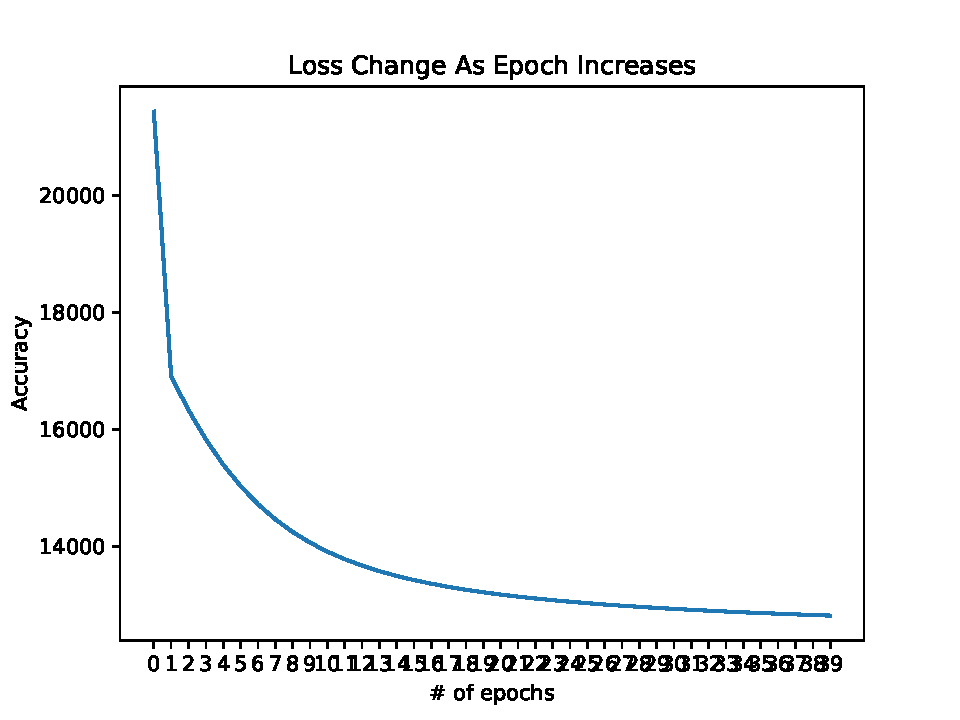
\includegraphics[scale=0.7]{figures/generated/nn_Loss_Change_As_Epoch_Increases.pdf}

    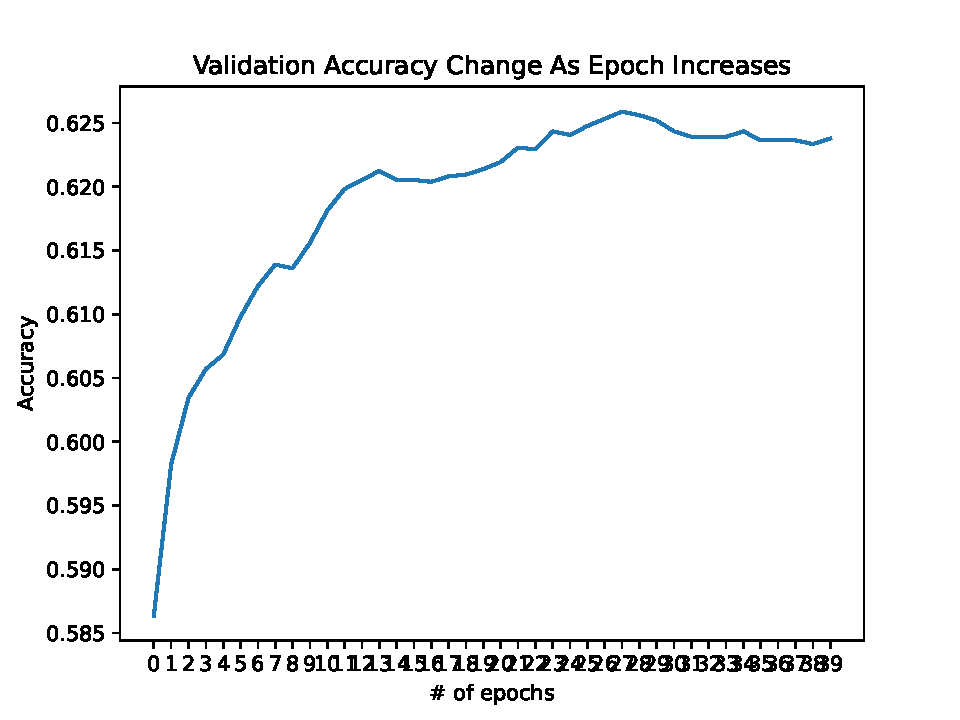
\includegraphics[scale=0.7]{figures/generated/nn_Validation_Accuracy_Change_As_Epoch_Increases.pdf}

    \subsection{Implementing $L_2$ Regularization}
    $L_2$ regularization has been implemented in the same code file as the other parts of this question (\verb|part_a/neural_network.py|).

    \begin{verbatim}
        lamb=0
        Final Validation Accuracy*    0.6858594411515665
        Final Test Accuracy*    0.6836014676827548
        lamb=0.001
        Final Validation Accuracy*    0.6869884278859724
        Final Test Accuracy*    0.6785210273779283
    \end{verbatim}

    \begin{verbatim}
        (optional extra finding):
        but with lamb=0.00025
        Final accuracy    0.6848715777589613
        Final Test Accuracy*    0.6861416878351679
    \end{verbatim}

    There are improvements on the validation accuracy, but not on the test accuracy.


    \pagebreak

    \section{Ensemble}
    Code for the ensemble is implemented in \verb|part_a/ensembly.py|. We bagged our base neural network, k-Nearest-Neighbor, and Item-Response models with their previously discussed optimal hyper parameters.

    \begin{pylabblock}[ENSEMBLE]
        import ensemble as ensemble
        ensemble.evaluate_ensemble(verbosity=1, data_path="./data")
    \end{pylabblock}

    \medskip

    Output:

    \printpythontex[verb]

    \medskip

    We selected 3 base model: kNN, item response model and autoencoder, the bootstrapping phase is done with \verb|numpy.choice|, which samples n user v from the training sparse matrix uniformly, with replacement. To accomadate at least one entree per user and to maintain user order that is required in current version of evaluation functions, we concatenated all of our samples under the original \verb|train_matrix|. We generate 3 versions of bagged train matrix then train each basemodel respectively. For final prediction, we take the average of the predictions given by the 3 trained models, if the average of the value is greater than (or equal to) $0.5$, the prediction will be $1$, otherwise, it will be $0$. Our final result on test data showed the ensemble algorithm performed better than kNN, had very close performance to neural network, and performed a bit less than item response model. To elaborate, we see that the test accuracy for the ensemble is around $69.4\%$ while the neural network's testing accuracy is around $68.6\%$, $68.4\%$ and IRT is around $70.6\%$. The average (without weighing) of the latter three is around $69.2\%$ which aligns with the first, i.e, the ensemble of the three. We believe this is because bagging may reduce variance, but will not affect the bias. It would seem that the two under-performing models, kNN and NN, dragged the accuracy down, while IRT kept it up.

\end{document}